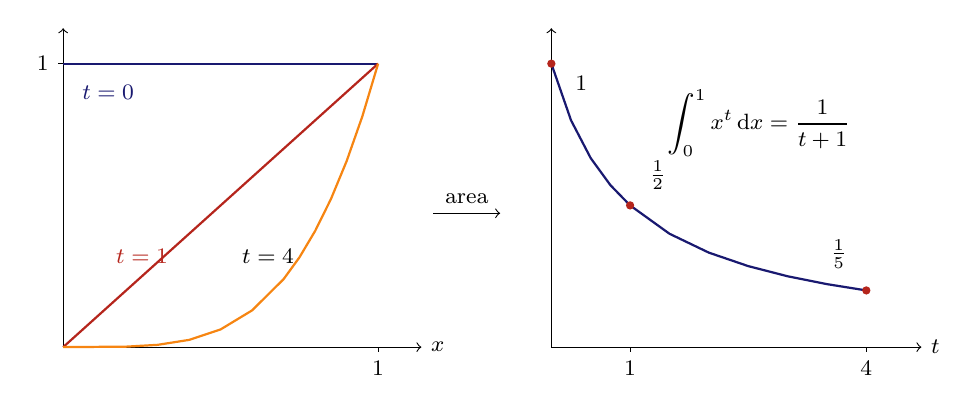
\begin{tikzpicture}[every node/.style={font=\footnotesize}]
  % Left: x |-> x^t on [0,1], drawn at 4 cm by 3.6 cm. The arrow carries the area to the right.
  \draw[->] (0,0) -- (4.55,0) node[right] {$x$};
  \draw[->] (0,0) -- (0,4.05);
  \draw (4,0) -- (4,-0.06) node[below] {$1$};
  \draw (0,3.6) -- (-0.06,3.6) node[left] {$1$};
  \draw[MidnightBlue,thick] (0,3.6) -- (4,3.6);
  \node[MidnightBlue,anchor=north west] at (0.12,3.45) {$t=0$};
  \draw[BrickRed,thick] (0,0) -- (4,3.6);
  \node[BrickRed,anchor=west] at (0.55,1.15) {$t=1$};
  \draw[BurntOrange,thick] (0.00,0.000) -- (0.80,0.006) -- (1.20,0.029) -- (1.60,0.092) -- (2.00,0.225) -- (2.40,0.467) -- (2.80,0.864) -- (3.00,1.139) -- (3.20,1.475) -- (3.40,1.879) -- (3.60,2.362) -- (3.80,2.932) -- (4.00,3.600);
  \node[black,anchor=west] at (2.15,1.15) {$t=4$};
  \draw[->] (4.70,1.70) -- (5.55,1.70) node[midway,above] {area};
  \begin{scope}[xshift=6.20cm]
    \draw[->] (0,0) -- (4.70,0) node[right] {$t$};
    \draw[->] (0,0) -- (0,4.05);
    \draw[MidnightBlue,thick] (0.00,3.600) -- (0.25,2.880) -- (0.50,2.400) -- (0.75,2.057) -- (1.00,1.800) -- (1.50,1.440) -- (2.00,1.200) -- (2.50,1.029) -- (3.00,0.900) -- (3.50,0.800) -- (4.00,0.720);
    \fill[BrickRed] (0,3.600) circle (1.5pt);
    \fill[BrickRed] (1,1.800) circle (1.5pt);
    \fill[BrickRed] (4,0.720) circle (1.5pt);
    \node[anchor=west] at (0.18,3.35) {$1$};
    \node[anchor=south west] at (1.12,1.88) {$\frac12$};
    \node[anchor=south east] at (3.88,0.88) {$\frac15$};
    \draw (1,0) -- (1,-0.06) node[below] {$1$};
    \draw (4,0) -- (4,-0.06) node[below] {$4$};
    \node[anchor=west] at (1.35,2.85) {$\displaystyle\int_0^1 x^{t}\,\mathrm{d}x=\frac{1}{t+1}$};
  \end{scope}
\end{tikzpicture}
